\documentclass[]{book}

%These tell TeX which packages to use.
\usepackage{array,epsfig}
\usepackage{amsmath}
\usepackage{amsfonts}
\usepackage{amssymb}
\usepackage{amsxtra}
\usepackage{amsthm}
\usepackage{mathrsfs}
\usepackage{color}
\usepackage{url}
\usepackage{tikz}
\usetikzlibrary{automata, positioning, arrows}


%Here I define some theorem styles and shortcut commands for symbols I use often
\theoremstyle{definition}
\newtheorem{defn}{Definition}
\newtheorem{thm}{Theorem}
\newtheorem{cor}{Corollary}
\newtheorem*{rmk}{Remark}
\newtheorem{lem}{Lemma}
\newtheorem*{joke}{Joke}
\newtheorem{ex}{Example}
\newtheorem*{soln}{Solution}
\newtheorem{prop}{Proposition}

\newcommand{\lra}{\longrightarrow}
\newcommand{\ra}{\rightarrow}
\newcommand{\surj}{\twoheadrightarrow}
\newcommand{\graph}{\mathrm{graph}}
\newcommand{\bb}[1]{\mathbb{#1}}
\newcommand{\Z}{\bb{Z}}
\newcommand{\Q}{\bb{Q}}
\newcommand{\R}{\bb{R}}
\newcommand{\C}{\bb{C}}
\newcommand{\N}{\bb{N}}
\newcommand{\M}{\mathbf{M}}
\newcommand{\m}{\mathbf{m}}
\newcommand{\MM}{\mathscr{M}}
\newcommand{\HH}{\mathscr{H}}
\newcommand{\Om}{\Omega}
\newcommand{\Ho}{\in\HH(\Om)}
\newcommand{\bd}{\partial}
\newcommand{\del}{\partial}
\newcommand{\bardel}{\overline\partial}
\newcommand{\textdf}[1]{\textbf{\textsf{#1}}\index{#1}}
\newcommand{\img}{\mathrm{img}}
\newcommand{\ip}[2]{\left\langle{#1},{#2}\right\rangle}
\newcommand{\inter}[1]{\mathrm{int}{#1}}
\newcommand{\exter}[1]{\mathrm{ext}{#1}}
\newcommand{\cl}[1]{\mathrm{cl}{#1}}
\newcommand{\ds}{\displaystyle}
\newcommand{\vol}{\mathrm{vol}}
\newcommand{\cnt}{\mathrm{ct}}
\newcommand{\osc}{\mathrm{osc}}
\newcommand{\LL}{\mathbf{L}}
\newcommand{\UU}{\mathbf{U}}
\newcommand{\support}{\mathrm{support}}
\newcommand{\AND}{\;\wedge\;}
\newcommand{\OR}{\;\vee\;}
\newcommand{\Oset}{\varnothing}
\newcommand{\st}{\ni}
\newcommand{\wh}{\widehat}

%Pagination stuff.
\setlength{\topmargin}{-.3 in}
\setlength{\oddsidemargin}{0in}
\setlength{\evensidemargin}{0in}
\setlength{\textheight}{9.in}
\setlength{\textwidth}{6.0in}
\pagestyle{empty}


\renewcommand{\thesection}{\arabic{section}}

\begin{document}

\tikzset{
->, % makes the edges directed
%>=stealth’, % makes the arrow heads bold
node distance=3cm, % specifies the minimum distance between two nodes. Change if necessary.
every state/.style={thick, fill=gray!10}, % sets the properties for each ’state’ node
initial text=$ $, % sets the text that appears on the start arrow
}

\begin{center}
{\Large Assignment 3}\\
\textbf{CSCE 4323: Formal Languages and Computability}

\textbf{Fall 2018}
%Due: DATE %You should write the date here.
\end{center}

\vspace{0.2 cm}


(Several of the following exercises can be found in Chapter 1 of the Sipser book, 2nd edition.)
Solutions for numbers 1, 1.46, and 1.53 should be neatly typed and submitted in PDF format. Soluctions for 1.6, 1.19, and 1.21 should be provided as code for each in a text document following the format for a regular expression or NFA, as appropriate, on the web site \url{http://web.cs.ucdavis.edu/~doty/automata/}. A template file ``CSCE4323-F18-HW-template.txt'' can be found on the course site on Blackboard.

\begin{thm}Regular languages are closed under complementation.\label{thm:comp}
\end{thm}

\begin{enumerate}

\item[1] Prove Theorem~\ref{thm:comp} (i.e. if $L$ is a regular language, then $\bar{L} = \Sigma^* \setminus L$ is also regular).

\item[1.6] Give regular expressions generating the following languages. In all parts, the alphabet is $\{0,1\}$.

    \begin{enumerate}
        \item[i.] $\{w |$ every odd position of $w$ is a $1\}$
        
        \item[j.] $\{w | w $ contains at least two $0$s and at most one $1\}$

    \end{enumerate}

\item[1.19] Use the procedure described in Lemma 1.55 to covert the following regular expressions to nondeterministic finite automata.

    \begin{enumerate}
        \item[a.] $(0 \cup 1)^*000(0 \cup 1)^*$
        \item[b.] $(((00)^*(11)) \cup 01)^*$
    \end{enumerate}

\item[1.21] Use the procedure described in Lemma 1.60 to covert the following finite automata to regular expressions.

    \begin{enumerate}
        \item[a.] 
        
            \begin{tikzpicture}
                \node[state, initial] (1) {$1$};
                \node[state, accepting, below=1] (2) {$2$};
                \draw 
                (1) edge[loop right] node{$a$} (1)
                (1) edge[below, bend left, right=0.3] node{$b$} (2)
                (2) edge[above, bend left, left=0.3] node{$b$} (1)
                (2) edge[loop right] node{$a$} (2);
            \end{tikzpicture}

        \item[b.]
        
            \begin{tikzpicture}
                \node[state, initial, accepting] (1) {$1$};
                \node[state, right of=1] (2) {$2$};
                \node[state, below left of=2, accepting] (3) {$3$};
                \draw
                (1) edge[above] node{$a,b$} (2)
                (2) edge[loop right] node{$a$} (2)
                (3) edge[below] node{$a$} (1)
                (3) edge[below
                , bend left, right=0.3] node{$b$} (2)
                (2) edge[above, bend left, right=0.3] node{$b$} (3);
            \end{tikzpicture}

    \end{enumerate}

\item[1.46] Prove that the following language is not regular.  You may use the pumping lemma and the closure of the class of regular languages under union, intersection, and complement.

    \begin{enumerate}
        \item[c.] $\{w|$ $w \in \{0,1\}^*$ is not a palindrome$\}$\footnote{A palindrome is a string that reads the same forward and backward.}
    \end{enumerate}
    
\item[1.53] Let $\Sigma = \{0,1,+,=\}$ and 

$ADD = \{x=y+z|$ $x,y,z$ are binary integers, and $x$ is the sum of $y$ and $z\}$.

Show that $ADD$ is not regular.

\end{enumerate}

\end{document}


